\documentclass[tikz]{standalone}
\usepackage{pgfplots}
\pgfplotsset{compat=1.15}
\usepackage{mathrsfs}
\usetikzlibrary{arrows,calc}
\usepackage{tkz-euclide}

\pagestyle{empty}

\definecolor{AngleClr}{rgb}{0,0.39215686274509803,0}
\definecolor{ShapeClr}{rgb}{0.6,0.2,0}
\definecolor{SecondAngleClr}{RGB}{14, 70, 161}

\begin{document}

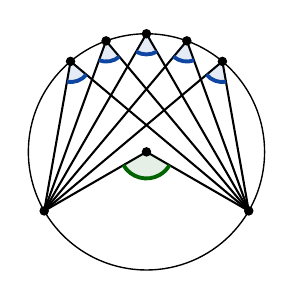
\begin{tikzpicture}[scale=.75]
\tkzSetUpLine[line width=1pt,color=black]
\tkzSetUpPoint[fill=black]

\tkzDefPoints{0/0/O,2/0/X}

\tkzDefPoint(-30:2){C}
\tkzDefPoint(210:2){A}
\tkzDefPoint(130:2){B1}
\tkzDefPoint(110:2){B2}
\tkzDefPoint(90:2){B3}
\tkzDefPoint(70:2){B4}
\tkzDefPoint(50:2){B5}

\tkzDrawCircle[color=black,fill=white,line width=0.5pt](O,X)

\tkzDrawSegments[line width=0.75pt,color=black](A,B1 C,B1 A,B2 C,B2 A,B3 C,B3 A,B4 C,B4 A,B5 C,B5 O,A O,C)

\tkzFillAngles[fill=SecondAngleClr,size=.35,fill opacity=0.1](A,B1,C A,B2,C A,B3,C A,B4,C A,B5,C)
\tkzMarkAngles[line width=1.4pt,size=.35,color=SecondAngleClr](A,B1,C A,B2,C A,B3,C A,B4,C A,B5,C)

\tkzFillAngles[fill=AngleClr,size=.45,fill opacity=0.1](A,O,C)
\tkzMarkAngles[line width=1.4pt,size=.45,color=AngleClr](A,O,C)

\tkzDrawPoints[size=3](A,B1,B2,B3,B4,B5,C,O)

% \tkzLabelPoint[below left](A){$\rm A$}
% \tkzLabelPoint[above left,scale=0.8](B1){$\rm B_1$}
% \tkzLabelPoint[above left,scale=0.8](B2){$\rm B_2$}
% \tkzLabelPoint[above,scale=0.8](B3){$\rm B_3$}
% \tkzLabelPoint[above right,scale=0.8](B4){$\rm B_4$}
% \tkzLabelPoint[above right,scale=0.8](B5){$\rm B_5$}
% \tkzLabelPoint[below right](C){$\rm\Gamma$}
% \tkzLabelPoint[above,scale=0.7](O){$\rm O$}


\end{tikzpicture}

\end{document}
